\label{sec:turbina}
\hspace{2cm}
\section{Prestazioni}



\begin{figure}[H]
    \centering

    \begin{minipage}[c]{0.62\linewidth}
        \centering
        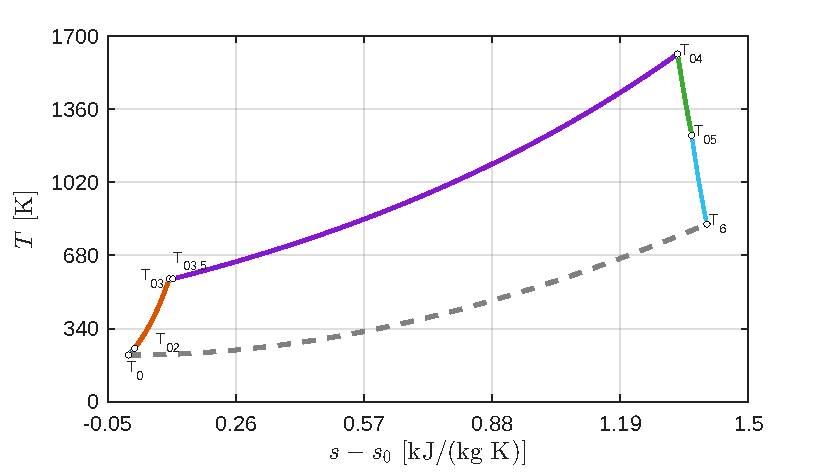
\includegraphics[width=\linewidth]
        {Graphics/turbogetto/prestazioni/ciclo.pdf}
        \caption{Rappresentazione del ciclo termodinamico del turbogetto.}
        \label{fig:prestazione:ciclo}
    \end{minipage}
    \hfill
\begin{minipage}[c]{0.34\linewidth}
    \centering

    \captionof{table}{Pressioni e temperature nei punti del ciclo.}
    \label{tab:pressioni}

    \fontsize{11pt}{11pt}\selectfont
    \renewcommand{\arraystretch}{1}
    \setlength{\tabcolsep}{3.5pt}

    \begin{tabular}{ccc}
        \toprule
        \textbf{Punto} & \textbf{$P$ [kPa]} & \textbf{$T$ [K]} \\
        \midrule
        $0$    & 19.2 & 216  \\
        $02$   & 29.4 & 248  \\
        $03$   & 406  & 571  \\
        $03.5$ & 394  & 571  \\
        $04$   & 371  & 1620 \\
        $05$   & 112  & 1240 \\
        $6$    & 19.2 & 825  \\
        \bottomrule
    \end{tabular}
\end{minipage}

\end{figure}

I principali risultati prestazionali ottenuti nel punto di progetto sono
riportati in Tabella~\ref{tab:prestazioni}.

\begin{table}[H]
\centering
\caption{Prestazioni principali del turbogetto, calcolate secondo la
procedura riportata in Appendice~\ref{appB:prestazioni}.}
\label{tab:prestazioni}
\fontsize{11pt}{11pt}\selectfont
\renewcommand{\arraystretch}{1}
\begin{tabular}{lrl}
\toprule
\textbf{Parametro} & \textbf{Valore} & \textbf{Unità} \\
\midrule
Spinta                    & 25.0  & kN \\
Spinta specifica          & 754 & m/s \\
TSFC                      & 0.135 & kg/(N$\cdot$h) \\
Rendimento propulsivo     & 41.2 & \% \\
Rendimento termodinamico  & 37.4 & \% \\
Rendimento globale        & 15.4 & \% \\
\bottomrule
\end{tabular}
\end{table}

La scelta di massimizzare la spinta specifica conduce a un valore di TSFC
superiore a quello di turbogetti ottimizzati prevalentemente sul consumo,
per i quali possono essere raggiunti valori inferiori a
$0.11\ \mathrm{kg/(N\,h)}$ \cite{Useller1954J71A2}. Tale risultato è
coerente con l'elevata temperatura di combustione adottata, che incrementa
la velocità di efflusso e quindi la spinta specifica, penalizzando al tempo
stesso il rendimento propulsivo \cite{slidesRobertoAndriani}.

\begin{table}[H]
\centering
\fontsize{11pt}{11pt}\selectfont
\renewcommand{\arraystretch}{1}
\caption{Portate massiche del turbogetto nel punto di progetto.}
\label{tab:mass}
\begin{tabular}{lrl}
\toprule
\textbf{Parametro} & \textbf{Valore} & \textbf{Unità} \\
\midrule
$\dot{m}_{\text{aria}}$         & 33.1 & kg/s \\
$\dot{m}_{\text{spillata}}$     & 3.23  & kg/s \\
$\dot{m}_{\text{combustibile}}$ & 0.938  & kg/s \\
$\dot{m}_{\text{totale}}$       & 34.1 & kg/s \\
\bottomrule
\end{tabular}
\end{table}

La portata d'aria richiesta risulta pari a $33.1\ \mathrm{kg/s}$, valore
ottenuto dall'ottimizzazione per soddisfare il requisito di spinta
contenendo al tempo stesso le dimensioni del propulsore. Di tale portata,
$3.23\ \mathrm{kg/s}$ vengono spillati dal compressore per il raffreddamento
della turbina, mentre la portata di combustibile risulta limitata a
$0.938\ \mathrm{kg/s}$.

Il modello introduce alcune semplificazioni, in particolare nella
modellazione della combustione e del raffreddamento della turbina, che
possono influenzare la stima delle prestazioni globali. La configurazione
ottenuta rispetta comunque i vincoli imposti durante l'ottimizzazione e
presenta dimensioni contenute, con raggio massimo all'ingresso della
turbina pari a $539\ \mathrm{mm}$. L'elevata spinta specifica favorisce
quindi una configurazione compatta, facilitando l'integrazione con il
ramjet nel sistema propulsivo complessivo.


































%----------------------------------------------------------------------------------------------------------------------------


%Risultano esserci inoltre alcune inefficienze e semplificazioni che dovrebbero essere prese in considerazione in caso di sviluppi futuri e che dovrebbero essere modificate. In particolare l'angolo $\alpha$ ottimo non verificato per la turbina, dovuto all'ipotesi di tenere la velocità assiale costante.  Il raffreddamento della turbina, che presenta notevoli approssimazioni su tutto il sistema coinvolto, per semplicità non vengono discussi spillamenti extra per sottosistemi. (possiamo mettere anche il fatto che si posso aggiungere molti piu vincoli nel ottimizzazione)